\begin{frame}{Representation by Noumi}
  \vspace{-1cm}
  {
    \small
    \begin{align*}
      \frac{d\sigma}{dM_{\pi\Sigma}d\Omega_{n}} &=& \left| \bra{n_{\theta=0}\pi\Sigma} T_2(\bar{K}N_2, \pi \Sigma) G_0(\bar{K}, N_2) T_1(K^-N_1, \bar{K} N) \ket{K^-\Phi_{d}} \right|^2\\
      \mbox{(Factrization)} &\Rightarrow& \left| T_2(\bar{K}N_2, \pi \Sigma) \right|^2 \left| \int G_0(\bar{K}, N_2) T_1(K^-N_1, \bar{K} N) d^3p_{N} \right|^2\\
    \end{align*}
    \vspace{-15mm}\\
    \begin{align*}
      & G_0(\bar{K}, N_2) \mbox{:Green Function}\\
      & T_1(K^- N_1, \bar{K}N)
      \mbox{:Partical Wave Analysis {\tiny \href{https://www.sciencedirect.com/science/article/abs/pii/0550321377900025}{G. P. Gopal et al., Nucl. Phys. B {\bf 119}, 362 (1977).}} }\\
      & T_2(\bar{K} N_2, \pi \Sigma) =
      \frac{e^{i\delta^{I}}}{\sqrt{k_1}}\frac{\sqrt{{\bf Im}A^{I}-\frac{1}{2}|A^{I}|^2{\bf Im}R^{I}k_2^2}}{1-iA^{I}k_2+\frac{1}{2}A^{I}R^{I}k_2^2}\\
      & \mbox{ {\tiny \hspace{2cm} \href{https://arxiv.org/abs/0804.3479}{L. Lesniak, arXiv:0804.3479v1, 2008.}} }
    \end{align*}
  }
  \\
  
  \centering
  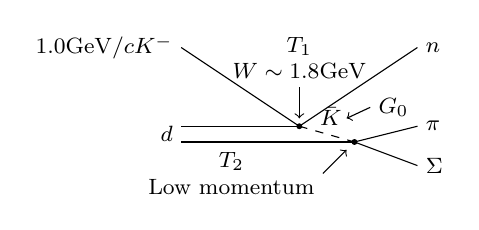
\begin{tikzpicture}[scale=1.0]
    \footnotesize
    \draw (-1.5,    1) node [left] {1.0GeV$/c $$K^-$}--(0,    0);
    \draw (-1.5,    0)--(0,    0);
    \draw (-1.5, -0.2)--(0.7, -0.2);
    \node (d) at (-1.5, -0.1) [left] {$d$};

    \draw (0, 0) -- (0.7, -0.2) [dashed];
    \node (barK) at (0.4, -0.1) [above] {$\bar{K}$};

    \draw ( 1.5,  -0.5) node [right] {$\Sigma$} -- (0.7, -0.2);
    \draw ( 1.5,  -0.0) node [right] {$\pi$}    -- (0.7, -0.2);
    \draw ( 1.5,  1.0) node [right] {$n$}      -- (0,    0);

    \draw [fill=black] (0, 0) circle (0.03);
    \draw [<-] (0.0, 0.1) to (0, 0.5) node [align=center, above] {$T_1$\\$W \sim 1.8$GeV};

    \draw [fill=black] (0.7, -0.2) circle (0.03);    
    \draw [<-] (0.6, -0.3) to (0.3, -0.6) node [align=center, left] {$T_2$\\ Low momentum};

    \draw [<-] (0.6, 0.1) to (0.9, 0.24) node [align=center, right] {$G_0$};
  \end{tikzpicture}
\end{frame}
